\documentclass[12pt]{report}

\usepackage{setspace}
\setlength{\parindent}{4em}

\usepackage{fancyvrb}
\usepackage{graphicx}
\usepackage{geometry}

\geometry{letterpaper, portrait, margin=1in}

%%%Title Page%%%
\title{
  Lab 06
\bigbreak Thunderbird Turn Signal with 1Hz Clock
}

\author{
{\normalsize
\begin{tabular}{l r r}
 & \textbf{Ryan Cruz} & \textbf{Zachary Davis}\\
\textbf{Category} & ryan.cruz25@uga.edu & zachdav@uga.edu\\
\hline
Pre-lab 						  & 50 & 50\\
In-lab Module \& Testbench Design & 50 & 50\\
In-lab Testbench Sim. \& Analysis & 50 & 50\\
In-lab FPGA Synthesis \& Analysis & 50 & 50\\
Lab Report Writing 				  & 50 & 50\\
\end{tabular}
}
}

\date{\bigskip
\today}
%%%%%%%%%%%%

\begin{document}
\maketitle

\section*{Lab Purpose}
	\paragraph{}
	The purpose of this lab is to continue and improve the execution of the previous lab, where we designed a finite state machine to control the taillights of a 1965 Ford Thunderbird using a physical switch to emulate the clock cycle. In this lab, we will leave the clock alone, but divide it by a considerable amount, so the LED refresh rate (AKA each clock cycle) can actually be seen by the human eye. The FPGA board we use has a 50MHz clock. To make this viewable, we will divide this so that the output on the board is 1Hz, or 1 second per clock cycle.
\section*{Implementation Details}
	\subsection*{Pre-Lab Design}
		\paragraph*{Finite-State-Machine}
			\hfill
			\begin{figure}[h]
				\centering
				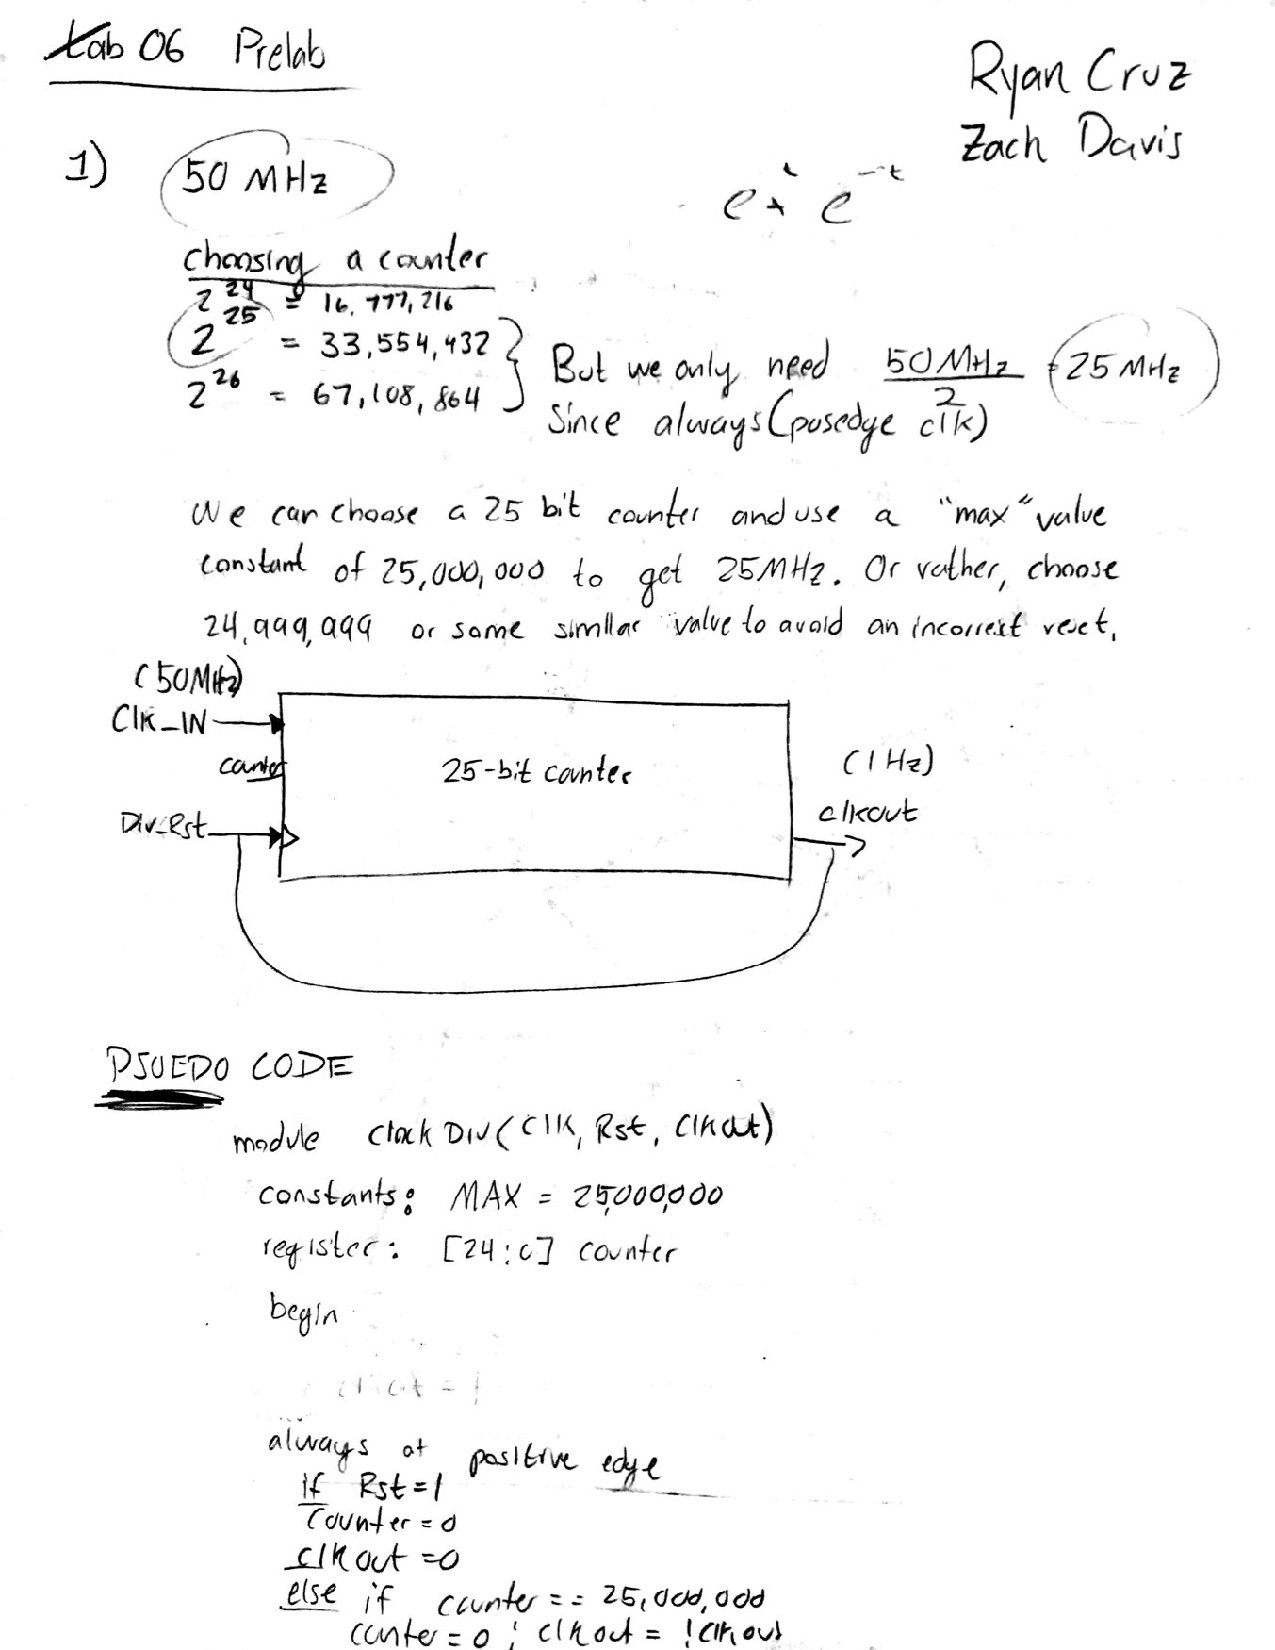
\includegraphics[scale=.44]{Prelab_6-page1.pdf}
				\caption{These are our ideas for implementing the clock divider, as well as some psuedo code to help us better imagine it in Verilog.}
			\end{figure}
			\newpage
			\begin{figure}[h]
				\centering
				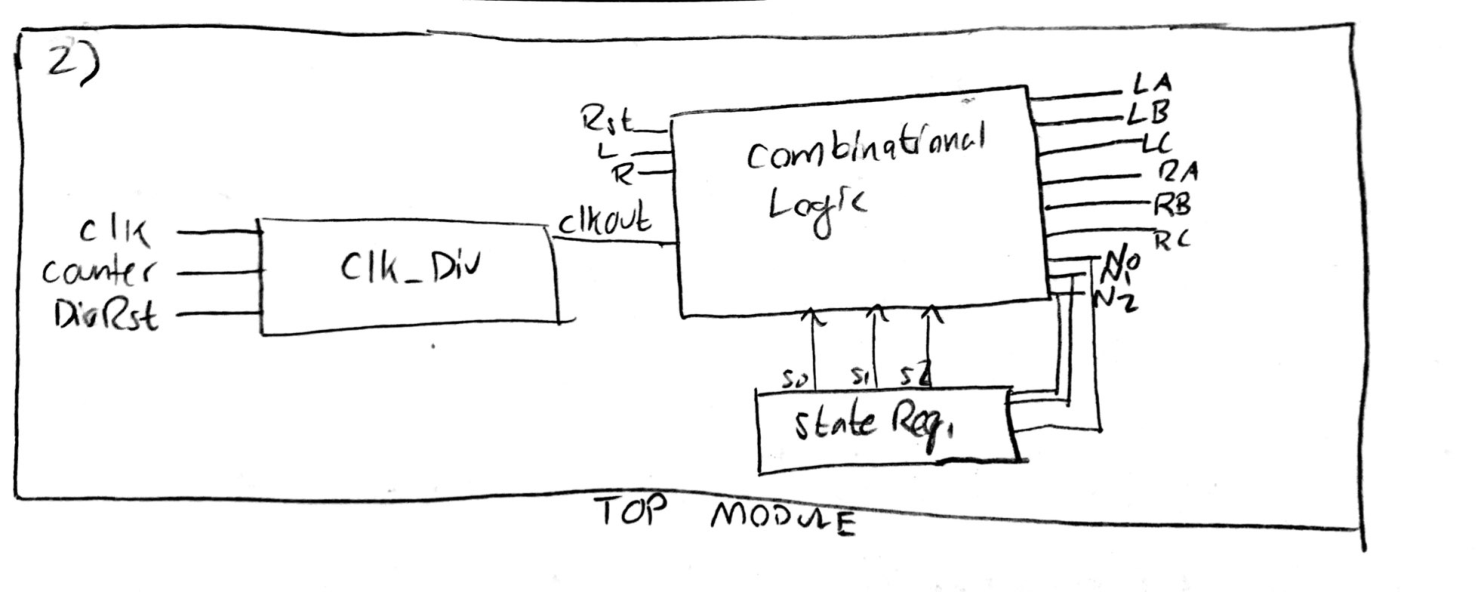
\includegraphics[scale=.44]{Prelab_6-page2.pdf}
				\caption{This is a schematic for the two parts of the code as well as the surrounding top module. The top module encapsulates all of the logic and the program can be run just as the top module. We made one edit to this schematic after taking a picture of it but before submitting it, which was adding a state register to the Clk\_Div portion, which is not seen here.}
			\end{figure}

	\subsection*{Clock\_Divider}
		\textbf{Behavioral Module Code}
		\begin{Verbatim}[frame=single, fontsize=\small]
`timescale 1ns / 1ps
////////////////////////////////////////////////////////////////////////////////
// Engineer: Zachary Davis
// 
// Create Date:    11:24:41 10/13/2017 
// Design Name:    Thunderbird Turn Signal
// Module Name:    Clock_Divider  
// Description:    A clock divider that divides 50 MHz into 1 Hz on the FPGA
//                 board.
//
////////////////////////////////////////////////////////////////////////////////
module Clock_Divider(Clk_In, Div_Rst, Clk_Out);
	input Clk_In, Div_Rst;
	output reg Clk_Out;
	reg [24:0] counter;
	
	always @(posedge Clk_In or posedge Div_Rst)
		begin
		if (Div_Rst == 1'b1)
			begin
			counter <= 0;
			Clk_Out <= 0;
			end
		else
			begin
			counter <= counter + 1;
			if (counter == 25_000_000)
				begin
				counter <= 0;
				Clk_Out <= ~Clk_Out;
				end
			end
		end
endmodule
		\end{Verbatim}
		
		\flushleft
		\textbf{Test Bench Code}
		\begin{Verbatim}[frame=single, fontsize=\small]
`timescale 1ns / 1ps
////////////////////////////////////////////////////////////////////////////////
// Engineer: Zachary Davis
// 
// Create Date:    11:24:41 10/13/2017 
// Design Name:    Thunderbird Turn Signal
// Module Name:    Clock_Divider_tb 
// Description:    A clock divider that divides 50 MHz into 1 Hz on the 
//                 FPGA board.  Simulator.
//
////////////////////////////////////////////////////////////////////////////////
module Clock_Divider_tb();
	reg Clk_In_s, Div_Rst_s;
	wire Clk_Out_s;
	
	Clock_Divider Clock_Divider_1(Clk_In_s, Div_Rst_s, Clk_Out_s);
	
	always
		begin
			Clk_In_s <= 1;
			#10;
			Clk_In_s <= 0;
			#10;
		end
	
	initial begin
		Div_Rst_s <= 0;
		#5;
		Div_Rst_s <= 1;
		#5;
		Div_Rst_s <= 0;
	end
endmodule

		\end{Verbatim}

	\newpage
	\subsection*{Thunderbird}
	\textbf{Behavioral Module Code}

		\begin{Verbatim}[frame=single, fontsize=\small]
`timescale 1ns / 1ps
////////////////////////////////////////////////////////////////////////////////
// Engineer: Zachary Davis & Ryan Cruz
// Create Date:    12:12:08 10/06/2017 
// Design Name:    Thunderbird
// Module Name:    Thunderbird.v 
// Project Name:   Thunderbird
// Target Devices: Spartan 3E
// Description:    Behavioral Design of the thunderbird blinker problem that
//                 was given in class.
//
// Revision: 
// Revision 0.01 - File Created
// Additional Comments: 
//
////////////////////////////////////////////////////////////////////////////////
module Thunderbird(L, R, Rst, Clk, LA, LB, LC, RA, RB, RC);
	
	//Define inputs and outputs of the circuit.  Using a 
	//3-bit register.
	input L, R, Rst, Clk;
	output reg LA, LB, LC, RA, RB, RC;
	reg [2:0] State, State_Next;

	//Defining all of the seven states from our FSM.
	parameter
		S_Off = 0,
		SL_On1 = 1,
		SL_On2 = 2,
		SL_On3 = 3,
		SR_On1 = 4,
		SR_On2 = 5,
		SR_On3 = 6;
		
//On every positive clock edge if reset is on then return to the off
//state, otherwise the current state equals whatever the next-state was
//defined as.
always@(posedge Clk)
begin
		if(Rst == 1)
			State <= S_Off;
		else
			State <= State_Next;
end

//Conditional Logic
always@(State, R, L, Rst)
	begin
		case(State)
			//Define all outputs at 0 before the first clock edge.
			default:
			begin
				LA <= 0; LB <= 0; LC <= 0;
				RA <= 0; RB <= 0; RC <= 0;
				State_Next <= S_Off;
			end
			
			//The off state has no lights on.  If neither R or L is 1
			//or R and L are 1 we remain in the off state as well as 
			//reset.  R or L being 1 initiates the blinker states.
			S_Off:
			begin
				LA <= 0; LB <= 0; LC <= 0;
				RA <= 0; RB <= 0; RC <= 0;
				if((Rst==0) && (R==0) && (L==1))
					State_Next <= SL_On1;
				else if((Rst==0) && (R==1) && (L==0))
					State_Next <= SR_On1;
				else if((R==1) && (L==1))
					State_Next <= S_Off;
				else if((R==0) && (L==0))
					State_Next <= S_Off;
				else 
					State_Next <= S_Off;	
			end
			
			//This is the first of three blinker states.  La is one
			//only.  If only R is on then the left cycle is ended 
			//and the right cycle is begun.  Both R and L being on 
			//or off do nothing by design.
			SL_On1:
			begin
				LA <= 1; LB <= 0; LC <= 0;
				RA <= 0; RB <= 0; RC <= 0;
				if((Rst==0) && (R==1) && (L==0))
					State_Next <= SR_On1;
				else if (((Rst==0) && (R==1) && (L==1)) 
						|| ((Rst==0) && (R==0)))
					State_Next <= SL_On2;
				else
					State_Next <= S_Off;
			end
			
			//This is the second of the three states.  This has the 
			//same properties as above.
			SL_On2:
			begin
				LA <= 1; LB <= 1; LC <= 0;
				RA <= 0; RB <= 0; RC <= 0;
				if((Rst==0) && (R==1) && (L==0))
					State_Next <= SR_On1;
				else if(((Rst==0) && (R==1) && (L==1))
						|| ((Rst==0) && (R==0)))
					State_Next <= SL_On3;
				else
					State_Next <= S_Off;
			end
			
			//The final left on state.  If R is one then the right 
			//cycle is begun otherwise its back to the off state.
			SL_On3:
			begin
				LA <= 1; LB <= 1; LC <= 1;
				RA <= 0; RB <= 0; RC <= 0;
				if((Rst==0) && (R==1) && (L==0))
					State_Next <= SR_On1;
				else
					State_Next <= S_Off;
			end
			
			
			//The same properties as the left counter part.
			SR_On1:
			begin
				LA <= 0; LB <= 0; LC <= 0;
				RA <= 1; RB <= 0; RC <= 0;
				if((Rst==0) && (R==0) && (L==1))
					State_Next <= SL_On1;
				else if(((Rst==0) && (R==1) && (L==1))
						|| ((Rst==0) && (L==0)))
					State_Next <= SR_On2;
				else
					State_Next <= S_Off;
			end
			
			//The same properties as the left counterpart.
			SR_On2:
			begin
				LA <= 0; LB <= 0; LC <= 0;
				RA <= 1; RB <= 1; RC <= 0;
				if((Rst==0) && (R==0) && (L==1))
					State_Next <= SL_On1;
				else if(((Rst==0) && (R==1) && (L==1))
						|| ((Rst==0) && (L==0)))
					State_Next <= SR_On3;
				else
					State_Next <= S_Off;
			end
			
			//The same properties as the left counterpart.
			SR_On3:
			begin
				LA <= 0; LB <= 0; LC <= 0;
				RA <= 1; RB <= 1; RC <= 1;
				if((Rst==0) && (R==0) && (L==1))
					State_Next <= SL_On1;
				else
					State_Next <= S_Off;
			end
		endcase
	end
endmodule
		\end{Verbatim}
	\textbf{Test Bench Code}
		\begin{Verbatim}[frame=single, fontsize=\small]
`timescale 1ns / 1ps
////////////////////////////////////////////////////////////////////////////////
// Engineer: Zachary Davis & Ryan Cruz
// Create Date:    12:12:08 10/06/2017 
// Design Name:    Thunderbird_tb
// Module Name:    Thunderbird_tb.v 
// Project Name:   Thunderbird
// Target Devices: Spartan 3E
// Description:    This simulates many cases of the thunderbird blinkers.  As 
//                 well as demonstrating how we handled some of the cases left
//                 to us.
//
// Revision: 
// Revision 0.01 - File Created
// Additional Comments: 
//
////////////////////////////////////////////////////////////////////////////////
module Thunderbird_tb();
	reg L_t, R_t, Rst_t, Clk_t;
	
	//Individually wiring each of the outputs.
	wire LA_t;
	wire LB_t;
	wire LC_t;
	wire RA_t;
	wire RB_t;
	wire RC_t;
	
	Thunderbird Thunderbird_1
	(L_t, R_t, Rst_t, Clk_t, LA_t, LB_t, LC_t, RA_t, RB_t, RC_t);
	
	//Setting the clock cycle frequency.
	always
	begin
		Clk_t <= 0;
		#10;
		Clk_t <= 1;
		#10;
	end
	
	//Manually testing all the cases of our design.
	initial
	begin
		//Initial input values.
		Rst_t <= 1;
		L_t <=0;
		R_t <=0;
		
		//Test the Left Blinker switch.
		@(posedge Clk_t);
		#5 Rst_t <=0;
		@(posedge Clk_t);
		#5 L_t <=1;
		@(posedge Clk_t);
		#5 L_t <=0;
		@(posedge Clk_t);
		@(posedge Clk_t);
		@(posedge Clk_t);
		
		//Testing the Right Blinker switch.
		@(posedge Clk_t);
		#5 R_t <=1;
		@(posedge Clk_t);
		#5 R_t <=0;
		@(posedge Clk_t);
		@(posedge Clk_t);
		@(posedge Clk_t);
		@(posedge Clk_t);
		
		//Testing Reseting the Left Blinker.
		@(posedge Clk_t);
		#5 L_t <=1;
		@(posedge Clk_t);
		#5 L_t <=0;
		@(posedge Clk_t);
		#5 Rst_t <=1;
		
		//Testing Reseting the Right Blinker.
		@(posedge Clk_t);
		#5 R_t <=1;
		#5 Rst_t <=0;
		@(posedge Clk_t);
		#5 Rst_t <=1;
		#5 R_t <=0;
		
		//Testing a Right Blinker Interrupting a Left Blinker.
		//Then A Left Blinker interrupting that Right Blinker.
		@(posedge Clk_t);
		#5 L_t <=1;
		#5 Rst_t <=0;
		@(posedge Clk_t);
		#5 L_t <=0;
		@(posedge Clk_t);
		#5 R_t <=1;
		@(posedge Clk_t);
		#5 L_t <=1;
		#5 R_t <=0;
		@(posedge Clk_t);
		#5 L_t <=0;
		@(posedge Clk_t);
		@(posedge Clk_t);
		@(posedge Clk_t);
		
		//Finally Testing Both Blinkers on and off.
		@(posedge Clk_t);
		#5 L_t <=0;
		#5 R_t <=0;
		@(posedge Clk_t);
		#5 L_t <=1;
		#5 R_t <=1;
		
		//Clearing the waves with a reset.
		@(posedge Clk_t);
		#5 L_t <=0;
		#5 R_t <=0;
		#5 Rst_t <=1;
	end
endmodule
		\end{Verbatim}
\subsection*{Top Module}
\textbf{Behavioral Module Code}
		\begin{Verbatim}[frame=single, fontsize=\small]
`timescale 1ns / 1ps
////////////////////////////////////////////////////////////////////////////////
// Engineer: Zachary Davis
// 
// Create Date:    11:24:41 10/13/2017 
// Design Name: 	 Thunderbird Turn Signal
// Module Name:    Top_Mod  
// Description: 	 Implements the thunderbird turn signal logic with a 
// a clock divider to implement in onto the FPGA Board.
//
////////////////////////////////////////////////////////////////////////////////
module Top_Mod(L, R, Rst, Clk_In, Div_Rst, LA, LB, LC, RA, RB, RC);
	input L, R, Rst, Clk_In, Div_Rst;
	output LA, LB, LC, RA, RB, RC;
	wire Clk_Out;
	
	Clock_Divider Clock_Divider_1 (Clk_In, Div_Rst, Clk_Out);
	Thunderbird Thunderbird_1 (L, R, Rst, Clk_Out, LA, LB, LC, RA, RB, RC);
endmodule

		\end{Verbatim}

		The \texttt{Top\_Mod} file simply combines the two other modules (\texttt{Clock\_Divider} and \texttt{Thunderbird}) by calling them. This is mainly for convenience, and it will become much more necessary when we have more than two modules in one verilog project.

\newpage
\section*{Experimental Results}

	\subsection*{Waveforms}
	\hfill
		\begin{figure}[h]
		\begin{center}
			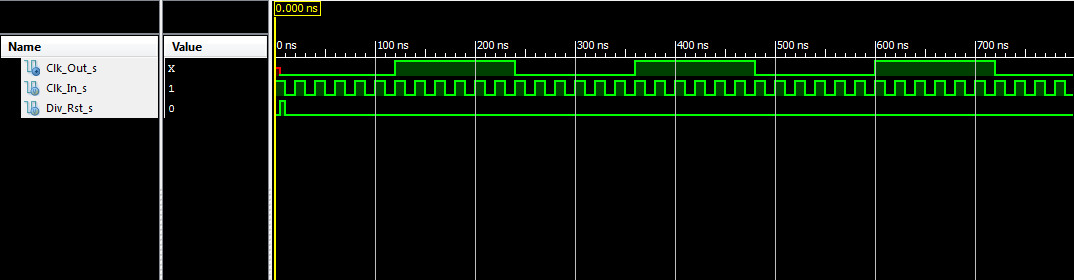
\includegraphics[scale=.55]{tb_5.PNG}
			\caption{This waveform shows the clock divider converting a 50 MHz clock
			to a 5 mHz clock. So, our \texttt{Thunderbird} module would execute on every rising edge of the \texttt{Clk\_Out} wave (5MHz), rather than the \texttt{Clk\_In} wave (50MHz). This was not the desired clock for the Thunderbird blinkers
			and was not the clock frequency used in our demo.  We did this only for the 
			simulation to see that we could divide the clock cycle and reducing it to a 1 Hz 
			clock would not be visible on the simulation. The amount of time (1 full second) that would have to pass relative to the sheer size of our monitors would be far too large to view/screenshot.}

			\hfill
 
			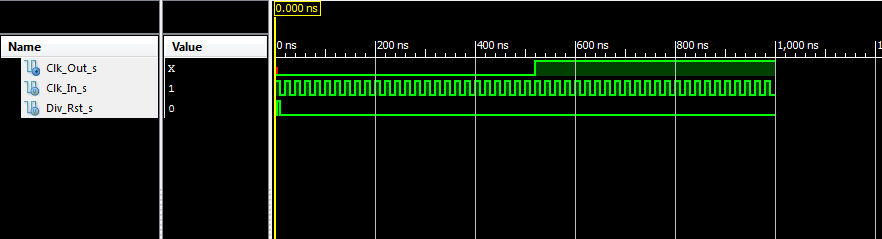
\includegraphics[scale=.67]{tb_25.PNG}
			\caption{This is the same clock divider with a different divider just to show again
			how it works in simulation, which would not be able to show 1 Hz against 50 MHz. The FPGA clock can be divided by basically anything to achieve the desired output for whatever case. If we had shown the actual conversion/division from 50 MHZ to 1Hz, $1*10^9$ nanoseconds would have to pass on this waveform graph.}
		\end{center}
		\end{figure}
\newpage
\section*{Significance}
	\paragraph{}
			Bouncing was the main issue with the previous implementation in Lab 05, also, clock division is a very common and useful tool to turn any clock frequency into something smaller. Specifically for us, we wanted to divide a large 50MHz clock into something viewable and distinguishable with the human eye. Using a simple clock division module in Verilog, we were able to elimate debouncing caused by the physical switch, as well as tune the frequency of our blinker to our liking. This makes tweaking and testing much easier, and the final product looks much cleaner. 
\section*{Comments/Suggestions}
	\paragraph{}
		We liked how this Thunderbird lab was split into two parts, but at the time of the demo of the \textit{first} lab, we were quite confused on what to do with the debouncing. We felt wrong for not implementing a software debounce, as we did not even know it would be a problem until the end of the first lab, where it was almost impossible to demo a perfect transition of states on the swithces, and then we learned it would be fixed in the next lab.
\section*{Additional Lab Information}
	\paragraph{}
		None necessary for this lab.
			
		
\end{document}

